%\IEEEraisesectionheading{\section{Introduction}\label{sec:introduction}}
\section{Introduction}\label{sec:introduction}
Designing \rts s is a challenging task as a growing requirements and expectations from systems. As Real time systems have to interact with real world entities most of the challenge comes from that. These interactions can get more and more complex. Typically a \rts might be interacting with thousands of such entities at the same time. For example, a telecom system routinely handles calls from thousands of people at the same moment. The system has to connect each call differently. Constraint like sequence of calls, amount of noise and quality of call availability of service etc.

For applications such as in air-traffic control system, satellite launching are considered as hard \rts because if deadlines which are not followed the system then it causes the catastrophic damage. For some other applications such as temperature reading response deadline is important but can be missed occasionally which is not desirable but not causing any catastrophic damage hence such applications are considered as soft \rts. Also some deadlines can start soft and later become hard. i.e., a $ 3 ms $ periodic reading on an aircraft pressure sensor is ideal but can be missed, however a $ 15 ms $ interval could cause catastrophe. A firm system such as weather forecast is one in which if the deadline is missed then no value for doing it later.

\begin{figure}[!htbp]
    \centering
    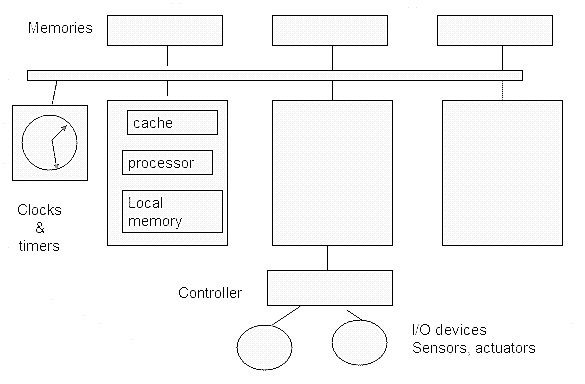
\includegraphics[width=0.5\textwidth]{genericsys.jpg}
    \caption{Generic Diagram of \rts\cite{realTimeIssues}}\label{fig:generic-rts}
\end{figure}

Components which are displayed in Fig. \ref{fig:generic-rts} are to be managed by program efficiently in such a way that maintains the accuracy of the system and achieve desire performance in terms of meeting deadline and response time.